\documentclass[crop, tikz]{standalone}
\RequirePackage{luatex85}

\usepackage{fontawesome}
\usepackage{fontspec}
\usepackage{ifthen}
\usetikzlibrary{
    backgrounds,
    patterns,
    mindmap,
    shapes,
    shapes.misc,
    fit,
    trees,
    tikzmark,
    arrows,
    arrows.meta,
    positioning,
    decorations.pathmorphing,
    shapes.geometric,
    decorations.pathreplacing
}

\newfontfamily{\ttfamily}{Fira Code}
\usepackage{fontspec}
\setmainfont{Liberation Sans}
\newfontfamily\ExtraLight{Liberation Sans}
\newfontfamily\Light{Liberation Sans}
\newfontfamily\Book{Liberation Sans}
\newfontfamily\Medium{Liberation Sans}

\definecolor{greenGood}{HTML}{99FF99}
\definecolor{redBad}{HTML}{FF9980}

\makeatletter
\tikzset{btree-key/.style={minimum height=1cm, pattern=north west lines, draw}}
\tikzset{btree-pointer/.style={minimum height=1cm, draw}}
\tikzset{btree-empty/.style={btree-pointer, dashed}}
\tikzset{btree-leaf/.style={fill=greenGood}}
\tikzset{btree-branch/.style={fill=gray!20}}
\tikzset{btree-line/.style={line width=0.5pt}}
\tikzset{btree-path/.style={btree-pointer, minimum width=0.5cm, fill=red, opacity=0.5}}
\tikzset{btree-hide/.style={draw opacity=0, line width=0, pattern=none}}
\tikzset{box/.style={draw, dashed, rounded corners, behind path}}
\tikzset{>=latex}

\newcommand{\btreenode}[5] {
    \path
      node[btree-pointer, #2, #3] (pointer1#1) {}
      node[btree-key, right=0 of pointer1#1, #3] (sep1#1) {}
      node[btree-key, left=0 of pointer1#1, #3] (sep2#1) {}
      node[btree-pointer, right=0 of sep1#1, #3] (pointer2#1) {}
      node[btree-pointer, left=0 of sep2#1, #3] (pointer3#1) {}
      node[btree-key, right=0 of pointer2#1, #3] (sep3#1) {}
      node[btree-key, left=0 of pointer3#1, #3] (sep4#1) {}
      node[draw, inner sep=0, behind path, #4,
          fit=(pointer1#1)(pointer2#1)(pointer3#1)
              (sep1#1)(sep2#1)(sep3#1)(sep4#1)
      ] (node#1) {};

      \ifthenelse{ \equal{#5}{show-pointers} } {
            \coordinate[below=0.5 of pointer1#1] (heap-pointer1#1);
            \coordinate[below=0.5 of pointer2#1] (heap-pointer2#1);
            \coordinate[below=0.5 of pointer3#1] (heap-pointer3#1);

            \draw[->, btree-line] (pointer1#1.south) -- (heap-pointer1#1.north);
            \draw[->, btree-line] (pointer2#1.south) -- (heap-pointer2#1.north);
            \draw[->, btree-line] (pointer3#1.south) -- (heap-pointer3#1.north);
      } {}
}

\makeatother

\begin{document}
    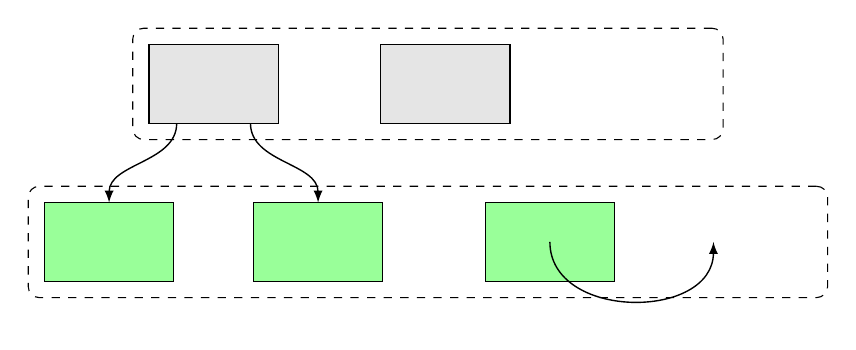
\begin{tikzpicture}[]
        \btreenode{1}{}{btree-hide}{btree-branch}{}
        \btreenode{2}{right=2cm of node1.east}{btree-hide}{btree-branch}{}
        \node[btree-hide, right=2cm of node2.east, minimum width=0.5cm] (node2-extra) {};

        \btreenode{3}{below=1cm of node1.south west, xshift=-0.5cm}{btree-hide}{btree-leaf}{}
        \btreenode{4}{below=1cm of node1.south east, xshift=0.5cm}{btree-hide}{btree-leaf}{}
        \btreenode{5}{right=2cm of node4.east}{btree-hide}{btree-leaf}{}
        \node[btree-hide, right=2cm of node5.east, minimum width=0.5cm] (node5-extra) {};

        \draw[->, btree-line] (pointer21.south)
            .. controls ([yshift=-1cm] pointer21) and ([yshift=1cm] pointer14) ..
            (pointer14.north);
        \draw[->, btree-line] (pointer31.south)
            .. controls ([yshift=-1cm] pointer31) and ([yshift=1cm] pointer13) ..
            (pointer13.north);

        \node[box, inner sep=0.2cm,
            fit=(node1)(node2)(node2-extra)
        ] (extent-1) {};

        \node[box, inner sep=0.2cm,
            fit=(node3)(node4)(node5)(node5-extra)
        ] (extent-2) {};

        \draw[->, btree-line] (node5.center)
            .. controls ([yshift=-1cm] node5) and ([yshift=-1cm,xshift=-1cm] node5-extra) ..
            ([xshift=-1cm]node5-extra.center);
    \end{tikzpicture}
\end{document}
